\section{Cours 4}
\subsection{Modélisation par flots}
L'objectif de la modélisation par flots est de:
\begin{itemize}
	\item modéliser des problèmes par des modèles de flots
	\item modéliser les problèmes de flots comme programmes linéaires
\end{itemize}

\textbf{Excès d'un sommet:\\}
L'excès du sommet v est le flot entrant dans v moins le flot sortant de v.

\textbf{Lemme:\\}
La valeur d'un flot est l'excès du sommet T, ou l'opposé de l'excès du sommet s.

\textbf{Théorème:\\}
$\forall$ flot f, et tout (s,t)-coupe (S,$\bar{S}$), val(f)$\leq$c(S,$\bar{S}$).\\
$\exists$ un flot f$^*$ et une (s,t)-coupe (S$^*$,$\bar{S}^*$) tels que val(f$^*$)=c(S$^*$, $\bar{S}^*$).\\
Alors, f$^*$ est un flot max, et (S$^*$, $\bar{S}^*$) une coupe minimum.

\textbf{Lemme:\\}
Si il existe une circulation avec demandes, alors $\Sigma_{v \in V}~d_v=0$, c'est à dire
$\Sigma_{v.d_v>0}~d_v=-\Sigma_{v:d_v<0}~d_v=:D$.

Le problème de flot de valeur d se réduit à la circulation eb posant d$_s$=-d, d$_t$=d, et d$_v$=0,
$\forall$v$\neq$s, t.
Le problème de circulation se réduit au flot max.

\subsection{Circulation et flots avec demandes et bornes inférieurs et bornes nip de capacités}
\begin{figure}[!ht]
	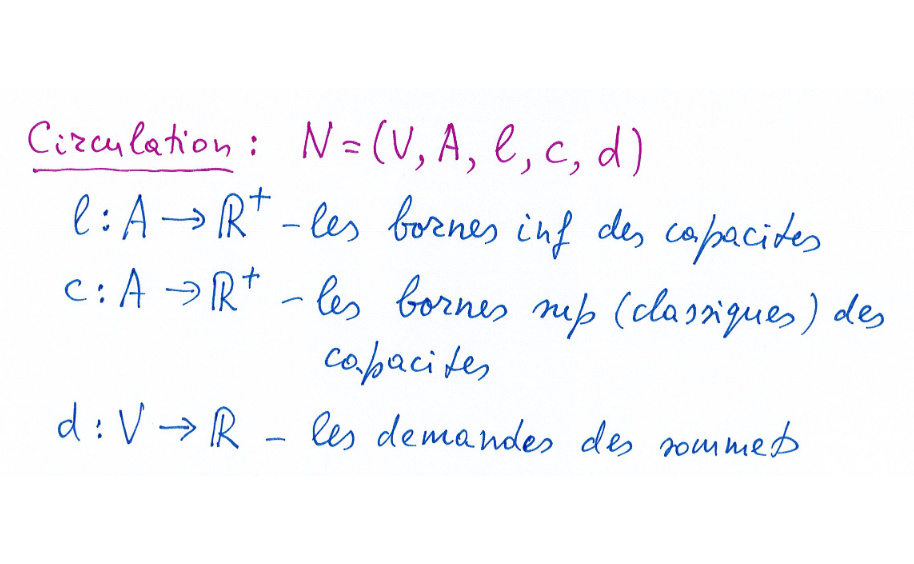
\includegraphics[width=\linewidth,height=0.75\textheight]{notes/algorithme/circu_flot.png}
	Si l($\overrightarrow{uv}$)=c($\overrightarrow{uv}$), cela oblige de passer par l'arc $\overrightarrow{uv}$ en
	quantité c=($\overrightarrow{uv}$).
\end{figure}
\begin{figure}[!ht]
	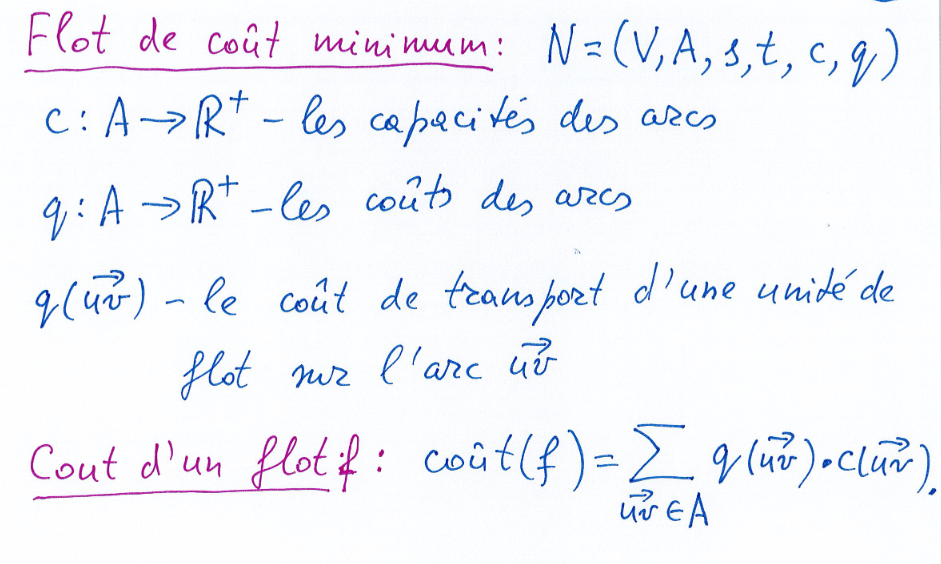
\includegraphics[width=\linewidth,height=0.75\textheight]{notes/algorithme/flot_min.png}
	Le flot de cout minimal généralize deux problèmes classiques:
	\begin{enumerate}
		\item le problème de transport
		\item le problème d'affectation
	\end{enumerate}
\end{figure}
\begin{figure}[!ht]
	\textbf{Problème de transport:\\}
	Déterminer, de façon optimale, l'acheminement des biens à partir de n entrepôts vers m destinataires.
	\begin{flushleft}
		\textbf{But:} Minimiser le coût de transport.
	\end{flushleft}
	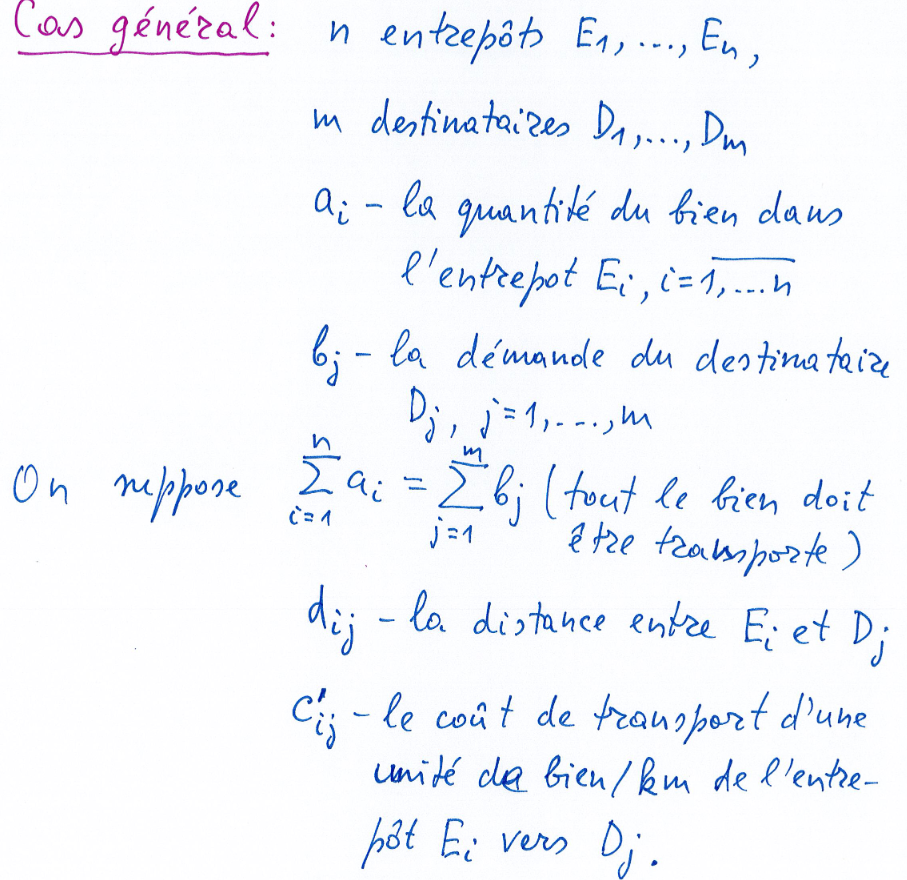
\includegraphics[width=\linewidth,height=0.75\textheight]{notes/algorithme/pb_trans_gen.png}
	\textbf{Le problème d'affectation:\\}
	n agents A$_1$...A$_n$ et n tâches T$_1$...T$_n$.\\
	Soit c$_{ij}$, le prix demandé par l'agent A$_i$ pour effectuer la tâche T$_j$.\\
	Chaque agent peux réaliser une seule tâche, et chaque tâche ne peut être réalisée que par un seul agent.\\
	\textbf{But:} Trouver une affectation de coût total minimal.
\end{figure}
\begin{figure}[!ht]
	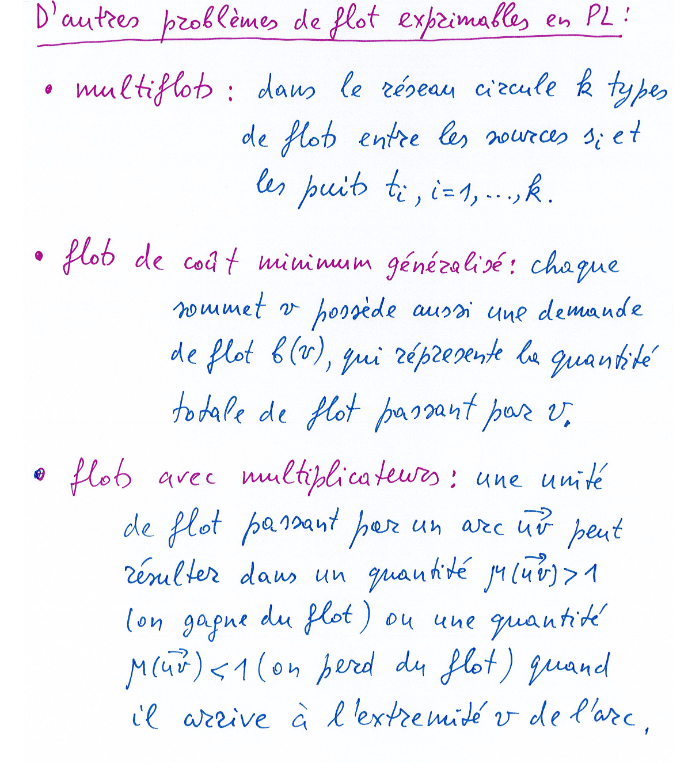
\includegraphics[width=\linewidth,height=0.75\textheight]{notes/algorithme/pb_exp_pl.png}
\end{figure}
